\documentclass[a4paper,11pt,twocolumn]{article}

\usepackage{xltxtra}
\usepackage{fontspec}

\defaultfontfeatures{Scale=MatchLowercase,Mapping=tex-text}

\usepackage{times}
\usepackage{natbib}

\usepackage[small,bf]{caption}


\setmainfont[BoldFont={Times New Roman}]{Times New Roman}
\setromanfont{Times New Roman}
%\setmonofont{FreeMono}


\bibdata{paper}


\title{A North Sámi to South Sámi machine translation prototype}
\author{Lene Antonsen,\\Giellatekno,\\Tromsø\\{\tt lene.antonsen@uit.no}
\and Francis Tyers,\\Giellatekno,\\Tromsø\\{\tt ftyers@dlsi.ua.es}
\and Trond Trosterud,\\Giellatekno,\\Tromsø\\{\tt trond.trosterud@uit.no}}
\date{}

\begin{document}

\maketitle


\begin{abstract}
This paper describes the development of a rule-based
machine translation system from North Sámi to South
Sámi, and its evaluation in a setting where North Sámi
functions as pivot translation via manual translation
from Norwegian North Sámi, and thereafter MT to South Sámi. 
\end{abstract}

\section{Introduction}
%@trond
%To be written after the paper is finished, but try to state the idea.

The paper presents a machine translation system from North Saami to
South Saami. The system is intended to work in a translation setting
where North Saami acts as a pivot language, with manual translation
from Norwegian into the largest of the Saami languages, and thereafter
to offer machine translation service, with postediting, to the other,
smaller, Saami languages. On the one hand, the Saami languages are
closely related, and therefore lend themselves better to MT than a
system translating from Norwegian directly, but on the other hand, the
classical problems of translating via a pivot language apply in this
case as well. 

The paper is structured as follows. Afther looking at previous work
and at the languages themselves, we give a presentation of the actual
machine translation system. Thereafter comes an evaluation of the
system. We presented translated text to translators, alongside with
the Norwegian original, without revealing the fact that the texts were
actually translated from North Saami.

finally comes a conclusion.


% Previous work
\cite{tyers09} \cite{wiechetek10} \cite{trosterud12}
% LREC for numbers for the sme-analyser:
\cite{AntonsenEtalReusing2010}

%pivot translation references --babych paper
\cite{babych2007}

\section{Languages}
%@trond
% [Sámi language area map]

As a Germanic language, Norwegian differs from the Saami languages
in numerous respects. It has definiteness as a morphological category,
no case, prepositions and verb / particle constructions, and a 
relatively strict word order, with V2 in main clauses. Norwegian
and the Saami languages also show Sprachbund phenomena, though.
Most notably, they have the same tense system. Whereas the Saami
languages also possess a number of infinite verb construction, the
Norwegian embedded clause pattern is in most cases a possible option
for the Saami languages as well.

The Saami languages constitute the westernmost branch of the Uralic
language family. They possess most of the classical Uralic
characteristica: A rich verbal morphology (3 numbers and persons, a
rich repertoire of infinite forms), and a medium-size case system with
both grammatical and adverbial functions, and no gender
distinction. They also show extensive contact with their Germanic
neighbours. Many grammatical structures are head-initial
constructions, as compared to the classical Uralic pattern, and the
tense system is compatible with the North Germanic one.

North and South Saami are not mutually intellegible, due both to
linguistic distance and to radically different prinicples for their
literary languages. An analogy would be the difference between English
and Frisian.

Grammatical similarities between North and South Saami include the
following: Both languages have 3 persons and numbers, they have a
similar system for postpositions and verb derivation. Noun phrase
syntax is similar, and the case systems are almost identical.

Taking a closer look, there are still differences. In both North and
South Saami, negation is expressed with a negation verb which inflects
for person and number, but in South Saami, this verb is inflected for
Tense as well. South Saami has OV word order and lacks a copula in
predicative constructions, whereas North Saami uses VO in simple
sentences, and requires a copula.  The possession construction is
different from the Norwegian one, normally using copula rather than
possessor subject + a verb \textit{to have}. In North Saami, the
construction is 
\textit{locative possessor + copula + possessed in nominative}, 
whereas the possessor is in the genitive in South
Saami.

Although the case systems are similar, North Saami has a locative case
that covers the semantic field of both inessive and elative in 
South Saami, the locative must thus be split into two cases. There is
also some differences in case usage, plural objects are accusative
in North Saami, but nominative for indefinite and accusative for 
definite objects in South Saami.

For a machine translation system the orthographic differences imply
that apart from person names and acronyms there will be no free rides
during the conversion process. The core vocabulary is distinct, even
recent loans from the same donor languages are different, and the
vocabulary coverage for a working system must thus be very good.

An overview over the differences between the two languages can
be found in \cite{sammallahti98}.


\section{Implementation}
%@fran

The translator was implemented using the Apertium platform \cite{forcada2011}. Apertium 
provides a highly modular set of tools for building rule-based
machine translation systems. Apertium language pairs are set up as Unix pipelines, where the
typical pipeline consists of:

\begin{itemize}
\item deformatting (encapsulating formatting/markup from the engine),
\item source-language (SL) morphological analysis with a finite-state
  transducer (FST),
\item disambiguation using a Hidden Markov Model (HMM) and/or
  Constraint Grammar (CG), 
\item lexical transfer (word-translation on the disambiguated source),
\item lexical selection (choosing the appropriate word out of a set of possible
   translations),
\item one or more levels of finite-state based structural transfer
  (reordering, and changes to morphological features),
\item target-language (TL) generation with an FST
\item reformatting (unencapsulating format information)
\end{itemize}

See Figure~\ref{fig:pipeline} for an overview of the modules used
in this particular language pair.

\begin{figure*}
 \centering
 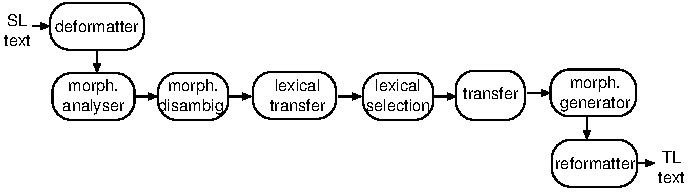
\includegraphics[width=0.75\textwidth]{architecture-overview.pdf}
 \caption{Overview of the translation pipeline.}
 \label{fig:pipeline}
\end{figure*}

\subsection{Analysis}

Morphological analysis is done on the input using the Helsinki Finite-State
Toolkit \cite{linden2011}. For each surface form, a finite-state transducer
returns a set of the possible analyses, where an analysis is a combination
of lemma, and a sequence of tags which describe the morphological structure
of the surface form.

A Constraint Grammar-based disambiguator then selects the most appropriate 
analysis for each surface form according to the context, and assigns to each 
analysis a syntactic tag denoting its syntactic function (subject, object, 
main verb, \ldots).

\subsection{Transfer}

\subsubsection{Lexical transfer}
%@lene

The bilingual dictionary: Some numbers 

\begin{itemize}
\item 3,568 general word pairs + 61 proper nouns
\item added: 873 special domain word pairs 
\item added: 10 721 proper nouns
\end{itemize}

There is no North Saami-South Saami dictionary, so we made one by making word pairs by combining the Norwegian words in a general North Saami-Norwegian dictionary and a general South Saami-Norwegian dictionary. The word pairs were manually edited and the work revealed many incorrect pairs because of Norwegian words with more than one meaning. Example is the Norwegian verb \textit{regne}, which means both 'to rain' and ‘to calculate’, which are two different verbs both in North Saami, \textit{arvit} and \textit{rehkenastit}, and in South Saami \textit{abrodh} and \textit{ryöknedh}. The result of this work was 3,568 general word pairs and 61 proper nouns.

The existing Norwegian-South Saami lexical resources are poor, with little terminology from the modern society. South Saami has been used more for giving information to the Saami people especially during the last two years, and there are some texts especially about school administration and curriculum on Internet. By comparing Norwegian texts with the translations to North Saami and South Saami, we added 873 special domain word pairs to the bilingual dictionary.

Large syntactic differences also have consequences for the bilingual dictionary, because many North Saami verbs have to be translated into South Saami as $object+verb$ and $adverb+verb$ strings. Examples include Norwegian `å trekke lodd', («draw lots for») which is translated into North Saami as one verb \textit{vuorbádit}, but into South Saami as object+verb \textit{vuerpiem giesedh} (lit. «lot draw»).
  
Norwegian `å presentere' is in North Saami \textit{ovdanbuktit} but in South Saami \textit{åvtese buektedh}. Often is the reason to this difference that one have utviklet North Saami terms to match the Norwegian terms, and in South Saami one still has to explain the meaning of the term with more words.

These are solved by adding giving the translation as MWE to the morpological analyser.



\subsubsection{Lexical selection}
Because we were adapting the MT system to a special domain, we only made xxx rules for lexical selection. An MT-system for more domains, will certainly need more such rules. 

The pivot model causes some extra lexical selection. Even if the lexical conceptualisation often is similar in South Saami and North Saami, as for the trivial ‘to rain, to calcute’ pair, there are also counter examples, like the Norwegian verbs \textit{lese, telle, uttale} ‘read, count, utter’, which all three can be expressed with the North Saami verb \textit{lohkat}. But in South Saami there is no common verb for these concepts, and the lexical distribution is like the one for Norwegian: \textit{lohkedh, ryöknehtidh, jiehtedh}. 


\subsubsection{Structural transfer}

The syntactic differences between North Saami and South Saami are
greater than are usually dealt with between related language pairs
in Apertium. 
In order to be able to transfer VO structures to OV more reliably,
the transfer phase is split into five parts instead of the three
more typically used in Apertium:

%t1x local chunking NP, VP
%t2x localcoordination NP+NP, etc.
%t3x empty, but for adpositional phrases + Rel clauses
%t4x Constituent mvm, SVO -> SOV
%t5x Cleanup

\begin{itemize} 
  \item \texttt{chunker}: Chunk input words into groups, e.g. noun groups, verb chains
  \item \texttt{interchunk1}: Merge chunks which have local coordination, e.g. the sequence [NP $x$] [CC and] [NP $y$] is merged into [NP $x$ and $y$]
  \item \texttt{interchunk2}: Merges relative clauses and adpositional phrases.
  \item \texttt{interchunk3}: Reorder constituents, e.g. SVO $\rightarrow$ SOV.
  \item \texttt{postchunk}: Cleanup
\end{itemize}

\subsubsection{Generation}

Generation is done using a finite-state transducer, also 
compiled using HFST. Each lexical unit which is output by
the postchunk module is looked up in the generation transducer
and the surface form is output.

\section{Evaluation}
%@ lene,fran
 translation nob-sma which actually is nob-sme-sma (should somehow be in the title?) 
 the evaluators evaluate nob-sma

\subsection{Statistics}
%@fran
\begin{table}
  \begin{center}
    \begin{tabular}{|l|r|}
      \hline
      Bilingual dictionary ({\tt sme}$\rightarrow${\tt sma}) & 15,204 \\ % 10776 proper names
      Transfer rules ({\tt sme}$\rightarrow${\tt sma}) & 57 \\
      \hline
    \end{tabular}
    \label{table:transfer}
    \caption{Number of bilingual dictionary entries and transfer rules}
  \end{center}
\end{table}

\begin{table}
  \begin{center}
    \begin{tabular}{|l|r|r|}
      \hline
      \textbf{Corpus} & \textbf{Tokens} & \textbf{Coverage (\%)}  \\
      \hline
      Schoolbooks     & 468,697 & 92.4 $\pm$ 0.58 \\
      General         & & 0.0 $\pm$ 0.0 \\
      \hline
    \end{tabular}
    \label{table:coverage}
    \caption{Vocabulary coverage of the system}
  \end{center}
\end{table}

\subsection{Quantitative}

WER -- word error rate
\begin{table}
  \begin{center}
    \begin{tabular}{|l|r|r|r|}
      \hline
      & \textbf{Eval. A} & \textbf{Eval. B} & \textbf{Eval. C}  \\
      \hline
\textbf{WER} (\%) & 62.37  &  49.46  &  52.69 \\
\textbf{PER} (\%) &  36.20   &  28.32  &  28.32 \\
      \hline
    \end{tabular}
    \label{table:coverage}
    \caption{Evaluation metrics.}
  \end{center}
\end{table}

\subsection{Qualitative}
%@lene

From the oovtast-presentation:
\begin{table*} 
\begin{center}
\begin{tabular}{|l|r||r|r|r|}
\hline
\textbf{ }  & \textbf{MT} &  \textbf{A} & \textbf{B} & \textbf{C} \\
\hline
Lexical differences: & &   37 & 27 & 19 \\
\hline
Morphological differences: & &   15 & 14 & 16 \\
\hline
\hline
\multicolumn{5}{|l|} {\textbf{Syntax} }   \\
\hline
SOV/SAdvlV & 4 &  10 & 12 & 12 \\
\hline
Det pronomen & 4 &   7 & 4 & 7 \\
\hline
Ind. articles & 0 &   7 & 0 & 1 \\
\hline
Complement instead of genitive mod. & -- &   2 & 2 & 0 \\
\hline
Habitive \textit{utnedh} & 0 &  5 & 2 & 2 \\
\hline
\hline
All together & 8 &   31 & 20 & 21 \\
\hline
\end{tabular}
\end{center}
\end{table*}

\subsection{User feedback}
%@lene

\section{Future work}
%@trond
\section{Conclusions}
%@trond

 reaction from sma linguist in the normgiving organ: she sees the possibility of using MT as a help for discussing terminology and getting the best ones into use

 the language socity is used to the impact from the mojority languages, a new controversial(?) thought is the linguistic impact from another minority lanugage 


\section*{Acknowledgements}

Linda Wiechetek, Divvun

\bibliographystyle{apalike}
\bibliography{paper}


\end{document}
